\section{Design}
\label{sec:design}

The design mainline are composed of ``Market Strategy'', ``System and Process'', and ``User Interface and Interaction'' to separate the business matters, logic elements, and display view.

% --------------------------------------------------
\subsection{Target User}

For our target user, strategy we're using is actually kind of concise. In the business related segment, it is by using what we call a \ac{BMC}\index{Business Model Canvas} to help shape the product which users would use up to customers would pay for.
More details on this can be seen in \autoref{chap:literature-study}.
Also as concerns of a wide range of market, Satellid implementation is not impartially refer to one of between the subject is a common vertical market (generally anyone, ordinary regular users and such) or diagonal market (specific types, from professionals to large industries).
Instead, we want to take a different approach.
We found and chose a what we came up with, a diagonal market which anyone can be just a user and even a paying customer.
This could cover both vertical and diagonal market within the same product.
Diagonal product can be too risky if we don't have a focus, so we first defined and validate the more likely to be considered which seems only be the users and customers.
The general ones are individuals and variety of teams.
The specific ones are students, educators, teachers, managers, creatives, developers, designers, entrepreneurs, software and information architect, strategy consultants, research analysts, organization managers, data analysts, \ac{CIO} and \ac{CTO} also even \ac{CEO}.
The culmination of this product is a general purpose type of tool that benefits both side of the worlds.
% [?] We can breakdown them each, later in the implementation chapter which also discuss the core features of what we're making.
But as explained in \autoref{sec:problem-scope}, we can't design for everyone in the beginning.
So we chose only for personal use who frequently gather and need to manage their knowledge at almost everytime.
Because we know what we design for, we can effectively start our design.
% [?] more words

% --------------------------------------------------
\subsection{Application Architecture}

As previously known, the application architecture is heavily based on Meteor platform.
It also covers its stack such as the JavaScript platform (Node.js), NoSQL database (MongoDB), reactive protocol (DDP).
All of them run in a regular web application environment, which there are client-side and server-side connected via a network that can be Internet or local network.
Based on simple web application architecture, the application is architected as in \autoref{fig:satellid-arch-app}.
% [?] inspired by

\begin{figure}[htbp]
    \centering
    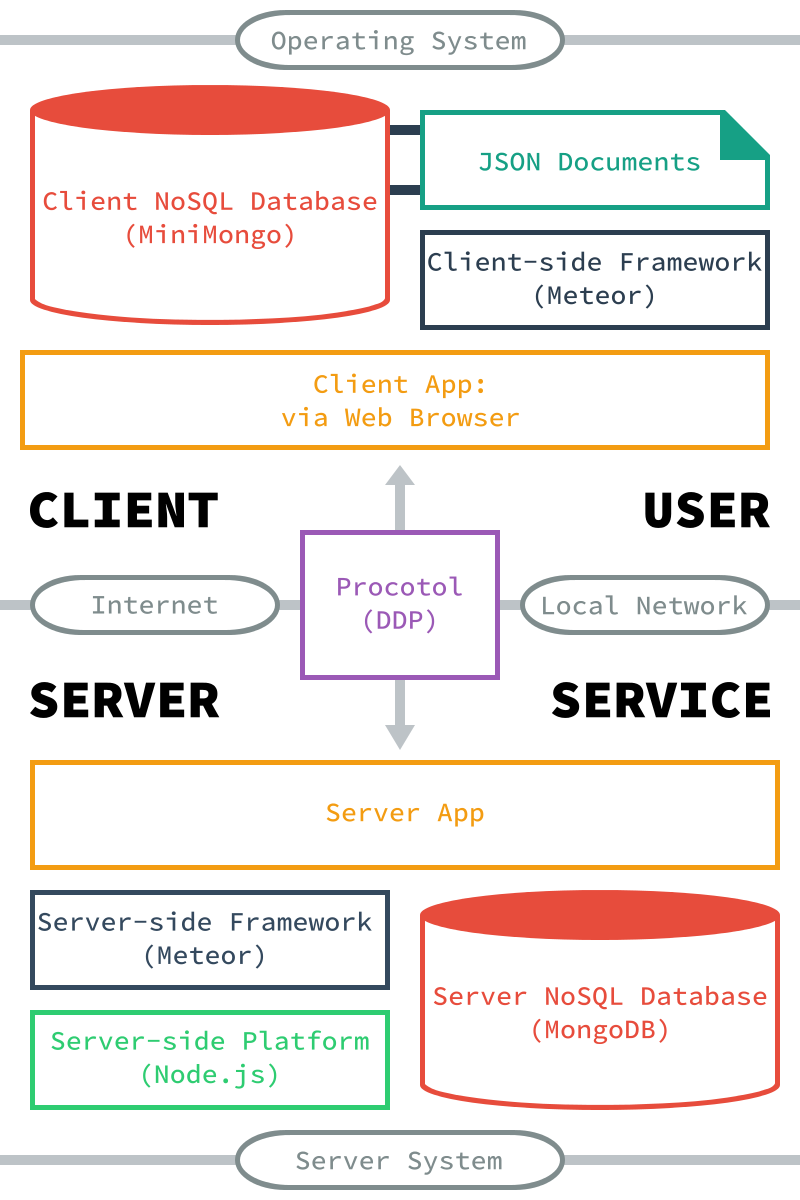
\includegraphics[width=8cm]{\dir/include/satellid-arch-app.png}
    \caption[Satellid Application Architecture]{The architecture of Satellid application}
    \label{fig:satellid-arch-app}
\end{figure}

The application started from the server system, running it including Node.js platform, Meteor platform, and server NoSQL database.
Those are served and accessed via the server-side app, naturally on top of a web server.
The application accessed by user from the client side, running it including Meteor app and client NoSQL database with \ac{JSON} documents that retrieved.
Those are accessible and enabled via client-side app, via the web browser.
Between the two, the protocol called \ac{DDP} maintain and manage the data transportation from server and client and from client to server.

% --------------------------------------------------
\subsection{User Interface and Interaction}

Here are the complete user interface and interaction on the web app version of Satellid.
The main interface or \ac{UI} design is laid out very simple, just like in \autoref{fig:satellid-ui}.

\begin{figure}[htb]
    \centering
    % \includegraphics[width=\textwidth]{\dir/include/satellid-ui}
    \caption{Main interface design of Satellid}
    \label{fig:satellid-ui}
\end{figure}

And then, the main interaction or \ac{UX} can be defined just like in \autoref{fig:satellid-ux}

%TODO User flow
\begin{figure}[htb]
    \centering
    % \includegraphics[width=\textwidth]{\dir/include/satellid-ux}
    \caption{Main interaction design of Satellid}
    \label{fig:satellid-ux}
\end{figure}

% --------------------------------------------------
\subsection{System and Process}

In the product segment, it is by shortening the steps that needed to do a knowledge management, with making it more effective and accessible.
Satellid uses an major role of feature called ``Contextual''.

\begin{figure}[htb]
    \centering
    % 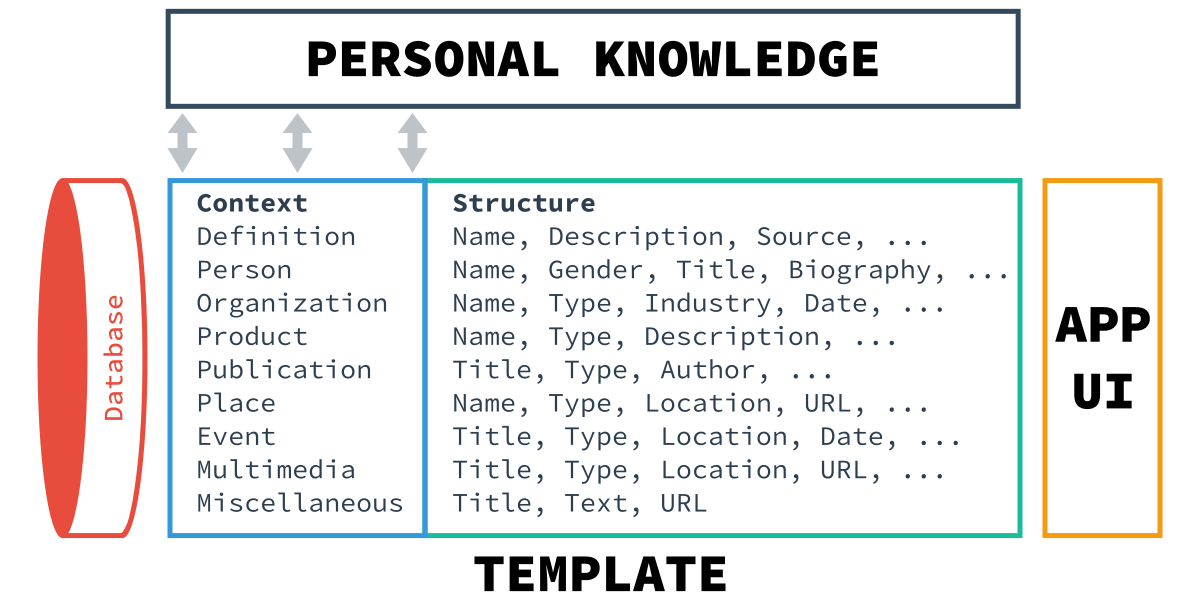
\includegraphics[width=\textwidth]{\dir/include/satellid-contextual}
    \caption{Contextual visual representation}
    \label{fig:satellid-contextual}
\end{figure}

Contextual, illustrated as in \autoref{fig:satellid-contextual}, utilize inputted knowledge and template that are used together to form the context and structure.
With this, user will eventually always structure their data, and even create more or modify available data field.
In addition to this, category and tagging could also be built.
At the later time, it can be easily sorted faster than just using category or tags.
The difference of context with category or tag is how it handles specificity.
Context is very specific as a descriptor so it can be fully understood and assessed easily, rather than category or tag that is more widely and freely determined.
For example, \textit{The Merriam-Webster Dictionary} may be categorized as a ``dictionary'', ``book'', ``reference'', ``glossary'', ``thesaurus'' and tagged as ``word'', ``language'', ``english'', ``''; but its context basically just a ``publication''.
So it can be in the same context like \text{JavaScript, The Definitive Guide} or even \text{Iron Man comic}.
Contextual provide some of the most common type of knowledge with its key attributes.
The basic properties of metadata are including ID, Context, Date \& Time (Created \& Updated); while others are the Content or Detail.
As already defined, the lists below are the sorted version of prospected key attributes related to single context that needed and can be used.
Each of them can have category or label if appropriate, even additional custom text.
Also sometimes blank field is allowed like if there is unknown location and URL, while in other condition multiple entries could occur.

\begin{easylist}
& Definition
  && Name, Description, Source URL
& Person
  && Name (Full, First, Last, Nick), Gender, Birth Date or Age, Title (Job), Biography, Location (Address \& Coordinates), Phone, Email, Website, URL
& Organization
  && Name, Type (School, University, Institution, Company, Group, Community, Band), Industry, Date (Founded), Location (Address \& Coordinates), Product (their Services or Goods), URL
& Product
  && Name, Type (Service, Hardware, Software, Food, Clothing), Tagline, Description, Brand Detail, URL
& Publication
  && Title, Type (Article, Book, Paper, Dictionary, Novel, Tutorial, Comic, Website, Blog), Author, Description, URL
& Place
  && Name, Type (Station, Library, Park, Shop, Restaurant, Mall, Hotel, City, Country), Location (Address \& Coordinates), URL
& Event
  && Title, Type (Meetup, Seminar, Workshop, Conference, Festival), Location (Address), Date, Presenter, Sponsor, URL
& Multimedia
  && Title, Type (Photo, Image, Video, Film), Location, Date and Time (Published), Duration, Creator, URL
& Miscellaneous
  && Name, Text, URL
\end{easylist}

Other contexts that classified as miscellaneous or mixed are like Rules, Manifesto, Prerequisites, etc.

Based on the system and process
